%%%%%%%%%%%%%%%%%%%%%%%%%%%%%%%%%%%%%%%%%%%%%%%%%%%%%%%%%%%%%%%%%%% 
%                                                                 %
%                           RELATED WORK                          %
%                                                                 %
%%%%%%%%%%%%%%%%%%%%%%%%%%%%%%%%%%%%%%%%%%%%%%%%%%%%%%%%%%%%%%%%%%% 

\chapter{RELATED WORK}
\label{related-work}
%\resetfootnote %this command starts footnote numbering with 1 again.

\section{General discussions on provenance and research reproducibility}
\label{sec:reproducibility}
Jarvis in \cite{jarvis2010importance} talks about the importance of provenance in the context of journalism. 
%according to Tan et al \cite{tan2007provenance}, the provenance information discussed in this proposal falls into the category of workflow (or coarse-grained) provenance, where detailed transformation processes of specific pieces of data in the final publications are not captured. For example, the process of generating a table is captured, but not the process that leads to specific columns, rows or cells of the table, which includes data transformation details such as the aggregation function used and the deletion of outliers.

Donoho et al in \cite{donoho2009reproducible} pointed out that current computational science practice, unlike the well-established deductive science and empirical science, doesn't generate routinely verifiable knowledge due to the lack of mature responses to the ubiquity of error in science such as formal logic and mathematical proof for deduction, and statistical hypothesis testing and standardized reproducibility information for empiricism. Following Claerbout's idea that
\begin{quote}
	We publish not just computational results
	but also the complete software environment
	and data that generated those results.
\end{quote}
, Donoho et al developed the Wavelab package which contained a unified set of wavelet and time-frequency tools that reproduce all the calculations in the papers Donoho and his collaborators had written on computational harmonic analysis \cite{buckheit1995wavelab}. In \cite{donoho2009reproducible}, the authors mentioned that reproducible publication packages benefit \emph{strangers} who don't possess our current short-term memory and experiences.
\begin{quote}
	In the heat
	of a computational project, we store many things
	in short-term memory that we need at that moment
	to use the code productively.
\end{quote}
In other words, conducting research in a reproducible manner hurts productivity in the heat of a project, although years from now, we ourselves, not remembering the myriad small details that accumulated in our minds during this project, will become such strangers.

Gentleman and Lang in \cite{gentleman2007statistical} proposed the idea of a \emph{research compendium}. A compendium can include several \emph{dynamic documents} that are mixtures of text and code. They also implemented a prototype by using a modified version of the \texttt{noweb} markup \cite{ramsey1994literate} to write dynamic documents, writing text chunks in a modified version of \LaTeX and writing code in R. Dynamic documents are processed with Sweave \cite{leisch2002sweave} and compendiums are represented as R packages.

Apparently, very few researchers have adopted the communication of research compendiums, as pointed out by Stodden in \cite{stodden2014enabling}. Most, if not all, of the problems listed in the \emph{Quick Answers to Knee-Jerk Objections} section of \cite{donoho2009reproducible} still remain in the way. For example, \emph{reproducibility takes time and effort}, although it may save us time in the long run. \emph{No one else does it, so I won't get any credit for it.} Creating compendiums instead of just papers really look wasting at the first sight. The list of problems goes on and on, and the cost of not working reproducibly is creeping and hurting really badly despite the fact that it is somewhat hard to work in this way. In her talk in 2011 \cite{stodden2011establishing}, Stodden argued that the lack of transparency is hurting the credibility of scientific research based on her observation in the field of statistics. Another evidence comes from the field of biomedical research, where Bustin in \cite{bustin2015reproducibility} pointed out that there is increasing concern about the reliability of biomedical research. It is estimated that up to 85\% of research funding is wasted in unreliable research.

This thesis provides a solution to reduce the time and effort required to create reproducible research publications. That is, the provenance capturing framework to be specified in Section~\ref{sec:framework} is for researchers who are willing to create reproducible publications but lack the knowledge and time to capture the necessary provenance.


%We plan to look further into the facts and references mentioned in this survey paper after proposal.

%The comment article introduces the series and discusses the consistent and colossal failure of initially promising research findings to translate into improvements in health care because of the many economic, political, social and cultural factors that influence researchers, funders, regulators, institutions and companies \cite{macleod2014biomedical}. 
%The first article in the series pointed out that the research studies supported by around US\$240 billion worldwide investment may have problems at the time funders decide what research to support, causing that much research does not lead to worthwhile achievements and that good research ideas do not yield the anticipated results \cite{chalmers2014increase}. 
%The second article in the series highlights that an absence of detailed written protocols and poor documentation of research is common and that inadequate emphasis is placed on recording of research decisions and on reproducibility of research \cite{ioannidis2014increasing}. 
%The third article discusses the modern approach to the regulation, governance, and management of biomedical research and emphasizes how inefficient management can easily compromise the interests of patients and the public \cite{salman2014increasing}. 
%The fourth article points out that a large percentage of protocols, reports and datasets associated with health research are rarely available, and there is selective reporting of methods and results, which leads to the introduction of bias and wastes huge amounts of research funding \cite{chan2014increasing}. The final article reemphasizes the absolute requirements for accurate, exhaustive and transparent reporting and notes that although reporting guidelines are important, they are all much less adopted and adhered to than they should be \cite{glasziou2014reducing}. The editors of the series make the revolutionary suggestion that rather than using journal impact factors to assess academics, it might be more reasonable to judge the researchers' work with the rigorousness of methodology, the transparency of reporting and the reproducibility of results, which would of course facilitate the publication of more reliable and biologically relevant data.


\section{Provenance capturing approaches}
Groth and Moreau in \cite{groth2009recording} presented five characteristics of high quality process documentation (that is, the provenance information) for results produced by distributed systems, namely \emph{immutable}, meaning intact after creation, \emph{attributable}, meaning clear responsibility, \emph{autonomously creatable}, meaning created by the most appropriate agent, \emph{finalizable}, meaning clear timing of completeness, and \emph{process reflecting}, meaning able to reflect the whole process leading to the final product. They also presented the concept of p-assertions first defined in their earlier work with others \cite{groth2006architecture} and the six key actors in provenance-aware systems, namely application, sender, receiver, asserter, recorder and provenance store. They described PReP --- the P-assertion Recording Protocol based on these actors and the model of applications as actors communicating via message passing. Groth and Moreau's approach is specially tailored for distributed computing scenarios, where actor model proposed by Agha et al.~\cite{agha1985actors,agha1997foundation} fits quite well. The framework specification of this thesis (see Section~\ref{sec:framework}) is based on the simple model of an application as a sequence of operation invocations carried out by operators. Our proof-of-concept prototype (to be described in Section~\ref{sec:prototype}) and case study (see Chapter~\ref{ch:case-study} for details) shows it is sufficient for research publication result preparation.

Miles et al. in \cite{miles2011prime} presents a provenance question driven methodology for developing provenance aware applications. The methodology decomposes the development process into three phases:
\begin{itemize}
	\item The \emph{use case identification} phase where provenance related requirements of the application are specified in terms of provenance questions and data items.
	\item The \emph{application decomposition} phase where the application is modeled in terms of actors and their interactions.
	\item The \emph{application adaptation} phase where the provenance capturing functions are engineered into the application.
\end{itemize}
The application is assumed to fit in the actor model, and the provenance captured is about interactions and actor state changes. We agree with Miles et al. that knowledgeable operators/actors, instead of a central provenance manager, are responsible for provenance capturing, so it is inevitable to adapt normal programs used by researchers to capture provenance about executions of these programs themselves. Discussion about the responsible operators of provenance is in Section~\ref{sec:framework}, and a sample adaptation of several frequently used research programs is presented in Section~\ref{sec:prototype} and the source code is listed in the appendix.

Workflow systems such as VisTrails \cite{freire2014reproducibility}, Kepler \cite{ludascher2006scientific}, Taverna \cite{wolstencroft2013taverna} and ReproZip \cite{chirigati2013reprozip} represent software components able to create data artifacts as \emph{program} nodes with input and output \emph{ports} connected with each other through \emph{channels}, as summarized in the ProvONE ontology\footnote{The ProvONE ontology. Available at http://purl.dataone.org/provone-v1-dev, accessed on November 18th, 2015.}. These systems allow reuse of workflows as long as the users are using the same system as the workflow creator. The provenance of a particular data artifact would be the specific \emph{execution} sequence of a set of programs. Program nodes in workflows are unified in terms of input and output ports so that they are more ready to get reused than normal programs. A workflow actually represents program components in a more intuitive way than a set of programs in the form of source code/binary files. Data provenance is a by-product rather than the major focus. Workflow creators could only record program execution related information and are limited on the additional information to add to the provenance graph.

\section{Provenance for research publications}
\subsection{Models for publication structure}
One important work on research publication structure modeling is the Document Components Ontology (DoCO), which is based on the rhetorical structure theory covered in \cite{taboada2006rhetorical}. This ontology integrated the SALT \cite{groza2007salt} (semantically annotates \LaTeX \ source files) ontology so that roles played by each part of the publication are made explicit. However, these roles are modeled as classes, which is against the fact that a role represents a relation between two entities. In the provenance ontology presented in this thesis, such roles are defined as properties to fit their relational nature, as will be described in Section~\ref{subsec:structure}.

Another model which is actively being developed now is nanopublications first proposed by Mons and Velterop~\cite{mons2009nano}. In this model, a nanopublication has three basic elements:
\begin{itemize}
	\item an assertion consisting of a subject, a predicate and an object,
	\item metadata providing contextual information about the assertion, and
	\item the publication information that is the metadata about the whole nanopublication.
\end{itemize}

The micropublications model proposed by Clark, Ciccarese and Goble in \cite{clark2013micropublications} extended statement-based models such as nano-publication by entities backing statements such as evidences and methods. In this model, a \emph{micropublication} argues \emph{claims}, which are supported by \emph{data}, other claims and \emph{attributions}, and data are produced by \emph{methods}.

The goal of our model for publication structure is to provide a way to describe and locate a published result in the context of a research publications, where \emph{results} could be in the form of figures, tables, lists and textual descriptions. We are more concerned about ``which section/chapter a certain figure is in'' than ``which statements support this claim'', so the abstract publication models such as nanopublications and micropublications do not fit our needs, while concrete models such as DoCO could serve well as a starting point to base our work.

%: a semantic model for claims, evidence, arguments and annotations in biomedical communications.

%And more to come after proposal...

\subsection{Models for Publication Preparing Process}
Although no models have so far specifically been designed for the generation process of published results, there are models for locating and tracking provenance for general information. The example is PML2~\cite{mcguinness2007pml}, of which the PML-P part models the concepts of \emph{information} and information container named \emph{source}. The ontology uses a ``raw string'' property to describe information content to deal with the heterogeneity of information, along with optional annotations such as ``language'', ``format'' and ``reference source usage'' (meaning how the information is obtained from a source). The process leading to some information is modeled in the PML-J part as inference steps generating conclusions based on antecedent conclusions and rules applied by inference engines. The model fits the scenario of semantic web agents drawing conclusions with rules, but is counter-intuitive for modeling data and results generated by operations.

Moreau et al. in \cite{moreau2011open} presented the Open Provenance Model (OPM), which provides a digital representation of provenance in terms of \emph{artifacts}, \emph{processes} and \emph{agents}. An OPM provenance graph contains facts of artifacts being generated by processes, which used (other) artifacts and was controlled by agents. Artifacts, processes and agents, along with their associated \emph{edges}, could belong to \emph{accounts} so that each account owns a subgraph that is a view of the whole provenance graph. The purpose of the OPM ontology (OPMO, and its successor PROV-O) is to represent provenance for any ``thing'', whether produced by computer systems or not. Therefore, this kind of general ontologies are good fits to base our work of modeling research publication result provenance on.

The W3C Provenance ontology PROV-O\footnote{http://www.w3.org/TR/prov-o/} shares a lot of elements with the OPM ontology\footnote{http://openprovenance.org/model/opmo}. PROV-O's \emph{entity}, \emph{activity} and \emph{agent} classes could find their matches \emph{artifact}, \emph{process} and \emph{agent} in the OPM ontology. Properties in PROV-O such as \emph{used} and \emph{was generated by} are modeled as \emph{edges} in OPMO and have the same names in the Open Provenance Model Vocabulary (OPMV, which is a lightweight version of OPMO). The \emph{used} and \emph{was generated by} (edge) classes in OPMO correspond to \emph{Usage} and \emph{Generation} classes in PROV-O. The major difference between PROV-O and OPMO+OPMV is that PROV-O replaced the edge class with the qualified classes and replaced properties associated with edge class instances with qualified properties. 

The W3C recommended PROV-O received wide adoption and efforts have been made to specialize it to fit a variety of domains and applications. D-PROV~\cite{missier2013d}
Costa et al.~\cite{costa2013capturing}
Belhajjame et al.\footnote{Wf4ever Research Object Model: http://wf4ever.github.io/ro/}

ProvONE\footnote{The ProvONE ontology. Available at http://purl.dataone.org/provone-v1-dev, accessed on November 18th, 2015.} integrated the work of Missier et al.'s D-PROV, Costa et al.'s and Belhajjame et al.'s Wf4ever. Although workflows are modeled as a type of programs, the ProvONE ontology uses workflow terms such as \emph{ports} and \emph{channels} to describe programs, so the scientific workflow community is likely to adopt the conceptualization of ProvONE quite readily. Figure~\ref{fig:provone} shows the major concepts defined in the ProvONE ontology.
\begin{figure}
	\centering
	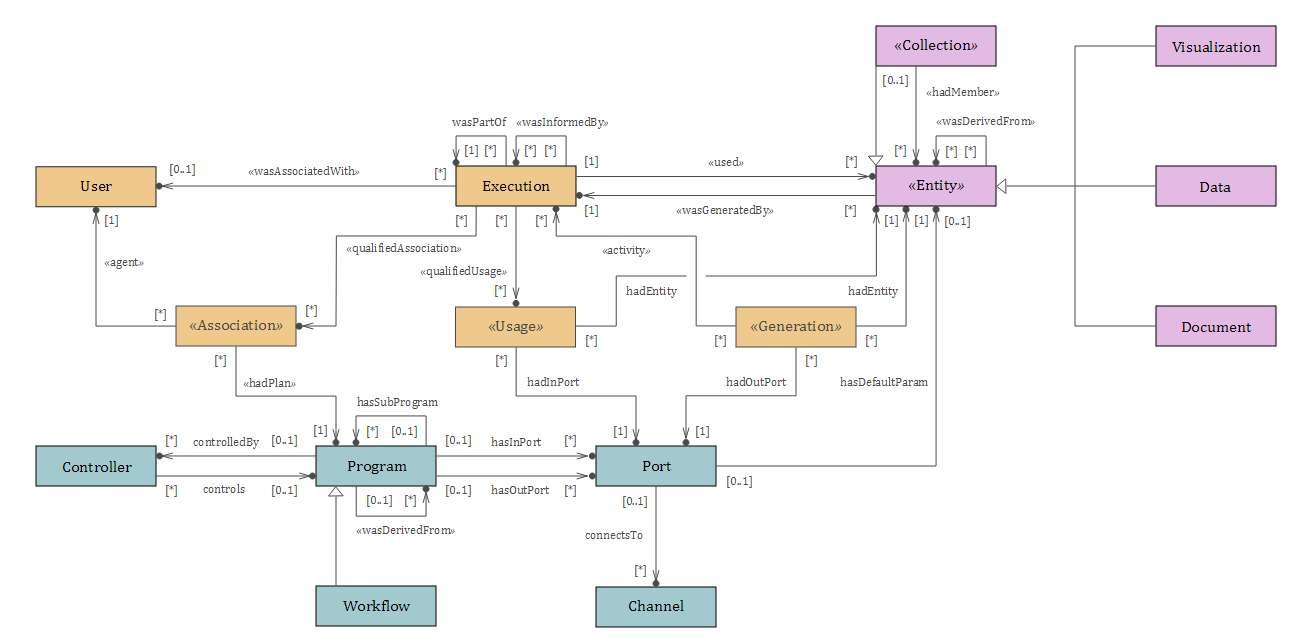
\includegraphics[width=\textwidth]{provone.png}
	\caption{ProvONE Conceptual Model UML Diagram}
	\label{fig:provone}
\end{figure}
In ProvONE, the \emph{Program} class is a subclass of prov:Plan
Different from the ProvONE model, our model does not include specific concepts for workflows: it describes any operation implementable with scripts in a certain programming language with properties \emph{pub:language} and \emph{pub:code}, and any other operation with property \emph{dct:description}. Actually pub:DataGeneration and pub:ResultGeneration could be asserted as subclasses of provone:Execution so that provenance graphs in PROV-PUB-O and ProvONE are interoperable: in ProvONE, code could be found in the \emph{Program} objects of the prov:hadPlan property of the prov:qualifiedAssociation property of \emph{Execution} objects; in PROV-PUB-O, code is the pub:code property of \emph{DataGeneration/ResultGeneration} objects, which are also \emph{Execution} objects. 

 %will be discussed in the final thesis.
Zhao et al.~\cite{zhao2006applying} about prospective and retrospective provenance

Freire et al.~\cite{freire2006managing} about process provenance or workflow evolution

\section{Ontology usability evaluation}
Ontology usability evaluation is an aspect of the more general task of ontology evaluation. As mentioned in \ref{subsec:evaluation}, ontology evaluation starts with checking completeness, consistency and conciseness of ontologies (e.g., \cite{gruninger1995methodology} and \cite{gomez2001evaluation}), so called \emph{deductive approaches} in 

To select an existing ontology to reuse in a new application, \emph{multiple-criteria approaches} (named by Brank et al in \cite{brank2005survey}) were developed. Ontologies are evaluated by several criteria and scores are given per criteria. An overall score of the ontology then could be calculated as the weighted sum of per-criteria scores. For example, Lozano-Tello et al presented the \emph{ONTOMETRIC} method in \cite{lozano2003selection,lozano2004ontometric}, which evaluates ontologies with a taxonomy of
160 characteristics organized in a multilevel framework. At the top level, there are five basic aspects. These are: 
\begin{itemize}
	\item the \emph{content} of the ontology and the
	organization of their contents,
	\item the \emph{language}
	in which it is implemented, 
	\item the \emph{methodology}
	that has been followed to develop it,
	\item the software \emph{tools} used to build and edit
	the ontology, and 
	\item the \emph{costs} that the ontology
	will be necessary in a certain project.
\end{itemize} 
As mentioned by Hartmann et al in \cite{hartmann2005d1}, this method requires a substantial amount of time to specify the relevant criteria and the scores are given quite subjectively.

Burton-Jones et al proposed an objective metric in \cite{burton2005semiotic}, where a set of 10 objective metrics at 4 different levels of a semiotic framework was presented. For example, at the \emph{syntactic} level, \emph{lawfulness} is defined as the total number of breached rules divided by the number of statements in the ontology, and \emph{richness} as the total number of syntactic features used in the ontology divided by the total number of available features in the ontology language. See Table 4 in \cite{burton2005semiotic} for the details of all the metrics. Since all the metrics used are objective, this approach does not require experts' review of the ontologies. However, the evaluation only gives the general quality of the ontology, which may have nothing to do with how well the ontology fits a certain task.

An really interesting work, although still not able to answer the ``how well it fits'' question, is \cite{gangemi2006qood}, where Gangemi et al organized the criteria for ontology evaluation and selection with a semiotic meta-ontology called $O^2$ and the \emph{oQual} evaluation ontology which involves concepts and relations relevant to ontology evaluation and selection. Therefore, evaluation based on the oQual ontology goes beyond the mere calculation of a weighted sum, but also contains reasoning based on the evaluation ontology. For example, the two criteria, namely \emph{explicitness} and \emph{computational efficiency} could be detected as conflicting by this approach because the former goal indicates high rate of cycles in the ontology but the latter indicates low rate of cycles. (See Figure 4 in \cite{gangemi2006qood} for the details.) Such a reasoning mechanism sheds more light than mere scores on the trade-offs to consider for the selection of ontologies.

The few work dealing with ontology usability evaluation includes \cite{casellas2009ontology}, which used System Usability Scale \cite{brooke1996sus} to evaluate the usability of the Ontology of Professional Judicial Knowledge (See Chapter 2 of \cite{casellas2009ontology} for a good introduction of the ontology).

%We also plan to look at the Severity Ratings for Usability Problems\footnote{http://www.nngroup.com/articles/how-to-rate-the-severity-of-usability-problems/ [Retrieved April 12th, 2015]}

%The approach we propose to develop is based on the intuition that better ontologies enable simpler software to accomplish a certain task, so we could evaluate the usability of ontologies by looking at the complexity of necessary software based on them.
%%% Local Variables: 
%%% mode: latex
%%% TeX-master: t
%%% End: 
